% arara: pdflatex
% arara: biber
% arara: pdflatex

\documentclass[a4paper]{article}
\usepackage[lighttt]{lmodern}
\ttfamily

% this is to fix a bug in the lmodern
\DeclareFontShape{OT1}{lmtt}{m}{it}
     {<->sub*lmtt/m/sl}{}
     
\usepackage[toc,page]{appendix}
%\usepackage{wrapfig}
\usepackage[pdftex]{graphicx}
%\usepackage[version=3]{mhchem}
\usepackage{fancyvrb}
%\usepackage{multirow}
\usepackage{url}
\usepackage{amsmath}
\usepackage{amssymb}
%package for this is ``algorithms''
\usepackage{algorithmic}
\usepackage{algorithm}
\usepackage{framed}

% this uses the IEEE naming conventions (apart from Procedure)
% \floatname{algorithm}{Procedure}
\renewcommand{\algorithmicrequire}{\textbf{Input:}}
\renewcommand{\algorithmicensure}{\textbf{Output:}}

% Making appendix work as part.
\usepackage{bookmark}


%\usepackage{threeparttable}
\author{Jim Finnis}

\newcommand{\todo}[1]{
    \begin{center}
    \fbox{\parbox{4in}{\textbf{To Do}\vspace*{1em} \\#1}}
    \end{center}}

\newenvironment{important}
{\begin{quote}\color{red}\large%
\begin{center}{\Large \textbf{IMPORTANT}}\end{center}}
{\end{quote}}

\newenvironment{notebox}[1][]
{\begin{framed}%
\ifthenelse{\equal{#1}{}}{}{%
    \begin{center}%
    {\Large \textbf{#1}}%
    \end{center}%
    }%
    }%    
{\end{framed}}


\DeclareMathOperator*{\argmin}{arg\,min}
\DeclareMathOperator*{\argmax}{arg\,max}
%\DeclareMathOperator*{\max}{arg\,max}
%\DeclareMathOperator*{\min}{arg\,max}
\DeclareMathOperator{\rand}{rand}
                                                                                           
% different commands for left and right margin notes                                                                                                   
\newcommand{\weeboxL}[1]{\rule{15mm}{0.5pt}\\ \parbox[t]{15mm}{\raggedright\footnotesize#1}}                                                                         
\newcommand{\weeboxR}[1]{\rule{15mm}{0.5pt}\\ \parbox[t]{15mm}{\raggedleft\footnotesize#1}}
                                                                                                                                                       
% this selects which command to use for margin notes                                                                                                   
\newcommand{\marg}[1]{\marginpar[\weeboxL{#1}]{\weeboxR{#1}}}

%\newcommand{\marg}[1]{\marginpar{\raggedright\footnotesize #1}}

% In math mode, put a word into text inside anglebrackets. Used for BNF, sometimes.
\newcommand{\angb}[1]{\text{$<$\\#1$>$}}

% so we can do 3\e{4} to do 3x10^4
\providecommand{\e}[1]{\ensuremath{\times 10^{#1}}}

\newenvironment{idescription}%
  {\begin{list}{}{\setlength{\labelwidth}{-10pt}
   \setlength{\itemindent}{-\leftmargin}
   \setlength{\listparindent}{\parindent}
   \renewcommand{\makelabel}{\descriptionlabel}}}%
  {\end{list}}


\DefineVerbatimEnvironment{v}{Verbatim}{
    %numbers=left,numbersep=5pt,
    %frame=lines,framerule=0.5mm,
    fontsize=\small,xleftmargin=15pt}
\DefineVerbatimEnvironment{vv}{Verbatim}{
    %numbers=left,numbersep=5pt,
    %frame=lines,framerule=0.5mm,
    fontsize=\small,xleftmargin=15pt}
\DefineVerbatimEnvironment{v2}{Verbatim}{
    %numbers=left,numbersep=5pt,
    %frame=lines,framerule=0.5mm,
    fontsize=\scriptsize,xleftmargin=0pt}
\DefineVerbatimEnvironment{v3}{Verbatim}{
    %numbers=left,numbersep=5pt,
    %frame=lines,framerule=0.5mm,
    fontsize=\tiny,xleftmargin=0pt}
\DefineVerbatimEnvironment{bv2}{BVerbatim}{
    %numbers=left,numbersep=5pt,
    %frame=lines,framerule=0.5mm,
    fontsize=\scriptsize,xleftmargin=0pt}
\DefineVerbatimEnvironment{bv}{BVerbatim}{
    %numbers=left,numbersep=5pt,
    %frame=lines,framerule=0.5mm,
    fontsize=\scriptsize,xleftmargin=0pt}
\DefineVerbatimEnvironment{bvc}{BVerbatim}{
    %numbers=left,numbersep=5pt,
    %frame=lines,framerule=0.5mm
    commandchars=+\[\],
    fontsize=\scriptsize,xleftmargin=0pt}

\setcounter{secnumdepth}{5}
\setcounter{tocdepth}{5}

%\usepackage[hmargin=2.5cm,vmargin=3.5cm]{geometry}
\usepackage[hmargin=3cm,
    vmargin=5cm,
    marginparwidth=2.0cm,
    ]{geometry}
\usepackage{multicol}
\usepackage{caption}
\usepackage{subcaption}
\usepackage{booktabs}
\usepackage{boldline}
\usepackage{multirow}
\usepackage{pdflscape}
\usepackage{afterpage}
\usepackage{amsmath}
\usepackage[all]{xy}
\usepackage{letltxmacro}
% uncomment this to enable internal automatic hyperlinks
\usepackage{hyperref}
\hypersetup{colorlinks}
\usepackage{listings}
\usepackage[usenames,dvipsnames]{color}
%Citation uses biber, and we set the style here
\usepackage[backend=biber,style=numeric,url=false]{biblatex}

\addbibresource{bib.bib}
\usepackage[font=small,labelfont=bf,margin=3em]{caption}
%\usepackage[LGR,T1]{fontenc}
%\newcommand{\textgreek}[1]{\begingroup\fontencoding{LGR}\selectfont#1\endgroup}
\usepackage{tikz}
%\usetikzlibrary{positioning}
\lstdefinelanguage{angort}{
morekeywords={for,if,then,else,leave,dup,call,global,swap,drop,not,
and,or,ifleave,const,over,defer,each,include,stop,dumplist,get,set,len,remove,shift,unshift,pop,push,map,reduce,filter,in,version,
barewords,dump,snark,none,p,x,rawp,nl,quit,debug,disasm,assertdebug,assert,assertmode,
abs,neg,isnone,gccount,range,srange,frange,frangesteps,i,j,k,iter,save,load,clear,
list,help,type,srand,rand,gc,format},
sensitive=false,
morecomment=[l]{\#},
morestring=[b]"
}
\lstdefinestyle{Python}{
  belowcaptionskip=1\baselineskip,
  breaklines=true,
  frame=L,
  xleftmargin=\parindent,
  language=Python,
  showstringspaces=false,
  basicstyle=\ttfamily\scriptsize,
  stringstyle=\slshape,
}
% patch fullcite to include the citation key
\LetLtxMacro\oldfullcite\fullcite
\renewcommand{\fullcite}[1]{\cite{#1}: \oldfullcite{#1}}

% This is a command to do subfigures easily. It's based on a
% stackoverflow hack : http://tex.stackexchange.com/questions/72902/new-command-with-variable-number-of-parameters
% The basic idea:
%
% The macro \twoimages really has no argument; it simply starts the
% business by opening the figure environment and calls the real command,
% \@twoimagesi. This command checks whether it's followed by
% \stopimages; if it is, it calls \@twoimagesend that ends the
% environment; otherwise it executes \@twoimagesii that has the job of
% printing a row, after having absorbed its six arguments. It does so in
% an indirect way, so that we can write only once the same minipage,
% using the first three arguments and the last three.
% Then \@twoimagesii restarts the recursion by calling \@twoimagesi again.
%
% Usage:
% \twoimages{caption}{label}
% {filename}{subcaption}
% {filename}{subcaption}
% {filename}{subcaption}
% \stopimages
%
% Labels will also be generated for each image, which are the filenames
% of the images.
%
% Optional command for image size multiplier

\makeatletter % we need to use kernel commands
\newcommand{\twoimages}[3][1]{%
  \def\jcf@tmpsiz{#1}
  \def\jcf@tmpcap{#2}
  \def\jcf@tmplab{#3}
  \begin{figure}[!htb]
  \@twoimagesi
}
\newcommand\@twoimagesi{\@ifnextchar\stopimages{\@twoimagesend}{\@twoimagesii}}

\newcommand\@twoimagesii[4]{%
  \@twoimagesiii{#1}{#2}\hfill
  \@twoimagesiii{#3}{#4}\\[\bigskipamount]
  \@twoimagesi % restart the recursion
}
\newcommand\@twoimagesiii[2]{%
  \begin{subfigure}{0.49\linewidth}
    \centering
    \includegraphics[width=\jcf@tmpsiz\textwidth]{#1}
    \caption{#2}\label{#1}
  \end{subfigure}}
\newcommand\@twoimagesend[1]{% The argument is \stopimages
  \vspace*{-\bigskipamount}
  \caption{\jcf@tmpcap \textit{(Label: \jcf@tmplab)}}\label{\jcf@tmplab}
  \end{figure}}
\makeatother

% similar but each line also takes a label
\makeatletter % we need to use kernel commands
\newcommand{\twoimageslabel}[3][1]{%
  \def\jcf@tmpsiz{#1}
  \def\jcf@tmpcap{#2}
  \def\jcf@tmplab{#3}
  \begin{figure}[!htb]
  \@twoimageslabeli
}
\newcommand\@twoimageslabeli{\@ifnextchar\stopimages{\@twoimageslabelend}{\@twoimageslabelii}}

\newcommand\@twoimageslabelii[6]{%
  \@twoimageslabeliii{#1}{#2}{#3}\hfill
  \@twoimageslabeliii{#4}{#5}{#6}\\[\bigskipamount]
  \@twoimageslabeli % restart the recursion
}
\newcommand\@twoimageslabeliii[3]{%
  \begin{subfigure}{0.49\linewidth}
    \centering
    \includegraphics[width=\jcf@tmpsiz\textwidth]{#1}
    \caption{#2}\label{#3}
  \end{subfigure}}
\newcommand\@twoimageslabelend[1]{% The argument is \stopimages
  \vspace*{-\bigskipamount}
  \caption{\jcf@tmpcap \textit{(Label: \jcf@tmplab)}}\label{\jcf@tmplab}
  \end{figure}}
\makeatother

% similar but each line is unlabelled
\makeatletter % we need to use kernel commands
\newcommand{\twoimagesnolabel}[3][1]{%
  \def\jcf@tmpsiz{#1}
  \def\jcf@tmpcap{#2}
  \def\jcf@tmplab{#3}
  \begin{figure}[!htb]
  \@twoimagesnolabeli
}
\newcommand\@twoimagesnolabeli{\@ifnextchar\stopimages{\@twoimagesnolabelend}{\@twoimagesnolabelii}}

\newcommand\@twoimagesnolabelii[4]{%
  \@twoimagesnolabeliii{#1}{#2}\hfill
  \@twoimagesnolabeliii{#3}{#4}\\[\bigskipamount]
  \@twoimagesnolabeli % restart the recursion
}
\newcommand\@twoimagesnolabeliii[2]{%
  \begin{subfigure}{0.49\linewidth}
    \centering
    \includegraphics[width=\jcf@tmpsiz\textwidth]{#1}
    \caption{#2}
  \end{subfigure}}
\newcommand\@twoimagesnolabelend[1]{% The argument is \stopimages
  \vspace*{-\bigskipamount}
  \caption{\jcf@tmpcap \textit{(Label: \jcf@tmplab)}}\label{\jcf@tmplab}
  \end{figure}}
\makeatother


% similar, but for three parallel images. More is just silly.


\makeatletter % we need to use kernel commands
\newcommand{\threeimages}[2]{%
  \def\jcf@tmpcap{#1}
  \def\jcf@tmplab{#2}
  \begin{figure}[!htb]
  \@threeimagesi
}
\newcommand\@threeimagesi{\@ifnextchar\stopimages{\@threeimagesend}{\@threeimagesii}}

\newcommand\@threeimagesii[6]{%
  \@threeimagesiii{#1}{#2}\hfill
  \@threeimagesiii{#3}{#4}\hfill
  \@threeimagesiii{#5}{#6}\\[\bigskipamount]
  \@threeimagesi % restart the recursion
}
\newcommand\@threeimagesiii[2]{%
  \begin{subfigure}{0.33\linewidth}
    \centering
    \includegraphics[width=\textwidth]{#1}
    \caption{#2}\label{#1}
  \end{subfigure}}
\newcommand\@threeimagesend[1]{% The argument is \stopimages
  \vspace*{-\bigskipamount}
  \caption{\jcf@tmpcap \textit{(Label: \jcf@tmplab)}}\label{\jcf@tmplab}
  \end{figure}}
\makeatother


% similar but takes any number of images and just puts them on subsequent lines at a given
% scale of the linewidth (the third argument).

\makeatletter % we need to use kernel commands
\newcommand{\multiimages}[3]{%
  \def\jcf@tmpcap{#1}
  \def\jcf@tmplab{#2}
  \def\jcf@tmpwidth{#3}
  \begin{figure}[!htb]
  \@multiimagesi
}
\newcommand\@multiimagesi{\@ifnextchar\stopimages{\@multiimagesend}{\@multiimagesii}}

\newcommand\@multiimagesii[2]{%
  \@multiimagesiii{#1}{#2} \\[\bigskipamount]
  \@multiimagesi % restart the recursion
}
\newcommand\@multiimagesiii[2]{%
  \begin{subfigure}{\linewidth}
    \centering
    \includegraphics[width=\jcf@tmpwidth\textwidth]{#1}
    \caption{#2}\label{#1}
  \end{subfigure}}
\newcommand\@multiimagesend[1]{% The argument is \stopimages
  \vspace*{-\bigskipamount}
  \caption{\jcf@tmpcap \textit{(Label: \jcf@tmplab)}}\label{\jcf@tmplab}
  \end{figure}}
\makeatother

% permits equation numbering in starred environments, so we can then
% label with \numberthis\label..

\newcommand\numberthis{\addtocounter{equation}{1}\tag{\theequation}}


\title{PCOT design notes}
\author{James Finnis (jcf12@aber.ac.uk)}

\begin{document}
\lstset{style=Python}
\maketitle
\LetLtxMacro\oldincludegraphics\includegraphics
% Stuff to redefine includegraphics to show the document file
% underneath; useful for referencing.
\renewcommand{\includegraphics}[2][]{%
%    \rotatebox[origin=tr]{270}{\tiny #2} %
    \oldincludegraphics[#1]{#2}%
    \\{\scriptsize #2}%
}



%Why is this even here?
%\nobibliography*
\tableofcontents


% Created by Jim Finnis
% Date Wed Feb 24 13:35:30 2021


\section{Introduction}
These notes provide some architectural details for PCOT to help
maintainers. I'll try to keep them up to date.

PCOT is based around a directed graph of nodes which perform
transformations of data. For this reason, the nodes are sometimes
called ``transforms'' and are represented by the \texttt{XForm} class
in the code.
Usually the data in question is an image, or rather an ``image cube'':
these have an arbitrary number of channels, not just the typical
RGB or greyscale. However, the data can be anything at all --- it depends
on the node. There is some typechecking when constructing the graph:
for exampel, you can't connect a ``rectangle'' output to an ``image'' input.
The entire application is shown in Fig.~\ref{app.png}. On the right
is a ``palette'' from which nodes can be selected to add to the graph,
while on the left
is an area which can show controls for each node in the graph, while
in the centre-right is the graph itself. This is shown in more detail
in Fig.~\ref{graph.png}.

\begin{figure}[ht]
\center
\includegraphics[width=6in]{app.png}
\caption{The PCOT application}
\label{app.png}
\end{figure}

\clearpage This will take an image from one of the data inputs --- these
exist independently of the graph proper and are configured with the four buttons
at the top of the window, see Sec.~\ref{inputs} ---
and perform a decorrelation stretch followed by a histogram
equalisation on the three channels selected in the \texttt{rect} node.
It will only do this to a rectangular
portion of the image (defined by the \texttt{rect} node), annotating the
region with some text defined in that node's controls. The
control region is currently showing the output of the histogram equalisation.

\begin{figure}[ht]
\center
\includegraphics[width=1.4in]{graph.png}
\caption{An example graph}
\label{graph.png}
\end{figure}


\subsection{Notes on type checking}
Python is dynamically typed, but there are a lot of ``type annotations''
in the code. Unfortunately, Python's import rules mean there's also some
odd stuff going on. Annotations like
\begin{lstlisting}
class XFormType:
    # name of the type
    name: str
    # the palette group to which it belongs
    group: str
    # version number
    ver: str
    # does it have an enable button?
    hasEnable: bool
\end{lstlisting}
are straightforward: we have three
string fields (\texttt{name}, \texttt{group} and \texttt{ver}) and
a boolean field (\texttt{hasEnable}). The next annotation, however,
is a link to a class defined further down the file, which in turn has
a field which is \texttt{XFormType}: a cyclic dependency. In such cases,
the standard PEP 0484 tactic is to use a string literal --- the type
checker will resolve this successfully and give appropriate warnings:
\begin{lstlisting}
    # all instances of this type in all graphs
    instances: List['XForm']
\end{lstlisting}
defines \texttt{instances} as a list of \texttt{XForm}.

Another oddity you may see in some of the files is this (from the top
of \texttt{xform.py} like the previous example):
\begin{lstlisting}
if TYPE_CHECKING:
    import PyQt5.QtWidgets
    from macros import XFormMacro, MacroInstance
\end{lstlisting}
These lines are only run when type checking, and are used to ensure
that appropriate classes are imported for type hints like this:
\begin{lstlisting}
    # an open help window, or None
    helpwin: Optional['PyQt5.QtWidgets.QMainWindow']
\end{lstlisting}
Without the \texttt{TYPE\_CHECKING} guard the program will not run, because
these imports are potentially cyclic. However, they are only needed at 
compile time, so the \texttt{if}-statement is added to stop the import
at run time. Note the quotes: they are there to stop Python trying to
resolve the symbols at run time.

\subsection{Structure}
The code is structured thus:
\begin{verbatim}
PCOT                    { main directory }
\-src                   { source code }
  \-pcot                { top-level package }
    \-assets            { data, typically .ui files }
     -calib             { code for handling colour calibration with PCT }
     -expressions       { expression parser package }
     -inputs            { data input method package }
     -operations        { "operations" package for node/expressions }
     -ui                { core user interface code and widget code }
     -utils             { utilities, e.g. archive managed, colour functions }
     -xforms            { the auto-registered XFormType node types }
\end{verbatim}
Notes:
\begin{itemize}
\item \textbf{operations} is a package for things which are both nodes and
expression functions, such as \emph{curve} and \emph{norm}: the operation
is encapsulated in a single function which is used by both a node
and a lambda for registering with the expression parser.
\item As well as containing the \texttt{src} directory, the top level
also contains files for installation and building single-file executables
with Poetry and PyInstaller.
\end{itemize}


% Created by Jim Finnis
% Date Wed Feb 24 13:48:57 2021


\section{The data model}
The data model consists of two parts --- the data itself (largely
image cube data) and the graph. By far the most important kind of data
from the point of view of this document is the image data, which ties
into the user interface in complex ways. Other forms of data do exist,
but these are much simpler.

\subsection{ImageCube}
Most classes making up the image data 
model are described in the \texttt{pancamimage.py} file, including the main \texttt{ImageCube}
class. Some additional classes describing where images can come from are in \texttt{channelsource.py}.
The model is shown in outline in Fig.~\ref{image.png} although some links to channel sources
and mapping from nodes are omitted; these will be explained later.

\begin{figure}[ht]
\center
\includegraphics[width=5in]{image.png}
\caption{Outline UML class diagram of image model}
\label{image.png}
\end{figure}

The main class is \texttt{ImageCube}: this encapsulates a numpy array
\texttt{img}
which is the actual image data cube in the form
of a $w \times h \times depth$ array. The data type is 32-bit floating
point, and images are typically normalized to the range [0,1].

\subsection{IChannelSource and implementations}
Each \texttt{ImageCube} has a number of channels, and for each channel there must be a corresponding
entry in the \texttt{sources} list. This describes where that channel came from, so that (typically) filter
information can be preserved, where appropriate, through the graph. The sources for each channel are a set
of \texttt{IChannelSource} objects. For example, if an image was loaded through the RGB loader, it might
have three ``fake'' channel sources for red, green and blue. Thus the sources will be 
\begin{v}
[ {RED}, {GREEN}, {BLUE} ]
\end{v}
i.e.\ a list of three sets, each with a single source.
If the image is then converted to greyscale, this could
become
\begin{v}
[ {RED,GREEN,BLUE}, {RED,GREEN,BLUE}, {RED,GREEN,BLUE} ]
\end{v}
because each channel now contains information from the red, green and blue channels in the source file.
The \texttt{RED}, \texttt{GREEN} and \texttt{BLUE} values refer in this case to \texttt{FileChannelSourceNoFilter} objects
which contain ``fake'' filter information and a filename identifier.
Each \texttt{IChannelSource} contains methods for accessing:
\begin{itemize}
\item an \textbf{identifier string} for the source from which the channel was acquired (typically a filename or data ID);
\item a \textbf{filter} and methods for obtaining the filter name, filter position and an actual filter reference (for extra data such as centre wavelength) (note
that much of this information will be ``fake'' for images loaded from plain RGB files);
\item methods for getting string descriptors for this source.
\end{itemize}

Nodes generate and process this information in different ways. For example, a ``gradient'' node takes a single channel and converts it into an RGB image with
a colour gradient: here, the output image's sources are ``internal RGB'' sources with no identifier or sensible filter data because the output's colour
is entirely artificial. In contrast, a the ``curve'' for performing a sigmoid function on all channels of an image will give the output image the
same sources as the input image.

Sources are used to keep track of each channel as it moves through the graph so they can be processed and displayed appropriately:
Fig.~\ref{app.png} shows a typical node in the ``node controls and output'' section. This section, as it does in many nodes,
contains a ``canvas'' displaying an image. Above the canvas are three combo boxes which select the channels in the image cube to display on the canvas,
and these are typically labelled by a string generated from the source data for each channel (along with the index).

\subsection{RGB mappings}


\subsection{Regions of interest}

% Created by Jim Finnis
% Date Wed Mar 3 15:15:17 2021


\section{Anatomy of an \texttt{XForm}: how to write nodes}
As noted above and shown in Fig.~\ref{xform.pdf}, all nodes are 
implemented as subclasses of \texttt{XFormType}. Each node 
is an \texttt{XForm} with a link to an \texttt{XFormType} object
controlling its behaviour\footnote{an example of ``favouring
composition over inheritance.''}.
There is only one object of each \texttt{XFormType} class; they
are singletons. The data differentiating each instance of 
a given node type is stored in the \texttt{XForm} itself.

To write a new node type we need to write a new \texttt{XFormType},
create a singleton object of that class, and register it with the system
(so the user can see it). The last two steps are dealt with automatically;
all we need do is write the class inside the \texttt{xforms} directory
and make sure it has the \texttt{@xformtype} annotation to ensure
it is registered and is a singleton, as described in 
Sec.~\ref{xformtype}.

In addition to an \texttt{XFormType}, it may be necessary to write
a subclass of \texttt{ui.tabs.Tab} to display its controls and output.
If the new node only displays
an image and has no extra controls, the built-in \texttt{TabImage}
can be used: I will discuss this case first.

\subsection{An example}
The required methods are described in Sec.~\ref{xformtype}. This
section will give an example of how to build an image manipulation
node --- an image normalisation node, which will normalise all channels
to the range [0,1]. It will also honour regions of interest:
only pixels inside the currently active ROI will be processed. This makes
image processing a little more complicated.

\subsubsection{Writing the operation}
We will be working in a file inside the \texttt{xforms} directory, which is
imported by \texttt{main.py}. We'll call this file \texttt{xformnorm.py}.
First, we need to write a function to normalise the image as a 3D numpy array,
taking into account a boolean mask of pixels to ignore (for the region
of interest). The declaration is simple:
\begin{lstlisting}
def norm(img, mask):
\end{lstlisting}
Now we need to generate a numpy masked array from the image and mask.
Note that the mask passed in uses True to indicate array elements which should
be used --- this is intuitively more obvious, but the construction
of a masked array uses True to indicate elements which are masked out. Thus
we need to negate the mask:
\begin{lstlisting}
    masked = np.ma.masked_array(img, mask=~mask)
\end{lstlisting}
Now we need to create a copy of the array to write the data to because we
don't want to modify the original image:
\begin{lstlisting}
    cp = img.copy()
\end{lstlisting}
Next we want to find the minimum and maximum of the pixels in the masked
image (i.e.\ ignoring unmasked pixels):
\begin{lstlisting}
    mn = masked.min()
    mx = masked.max()
\end{lstlisting}
If the range is zero, we generate an error --- we'll return this and deal
with it in \texttt{perform()}, our node's actual work function. We also
generate a zero image as the result.
If the range is OK, the exception is None and the result image is
the input image normalised
to the range of the masked pixels:
\begin{lstlisting}
    if mn == mx:
        ex = XFormException("DATA", "cannot normalize, image is a single value")
        res = np.zeros(img.shape,np.float32)
    else:
        ex = None
        res = (masked - mn) / (mx - mn)
\end{lstlisting}
We now put the result image into the image copy we generated earlier,
but this time we don't negate the mask (because \texttt{putmask} works
the right way --- pixels which are True in the mask are written). We 
then return the exception and the modified image copy.
\begin{lstlisting}
    np.putmask(cp, mask, res)
    return ex, cp
\end{lstlisting}
As you can see, error handling and dealing with regions of interest
is often the most complicated part of a node!
Now we can start to write the actual node class.
\subsubsection{The \texttt{XFormType} subclass}
As described above in Sec.~\ref{xformtype}, the behaviour of an \texttt{XForm} node is determined
by the \texttt{XFormType} singleton to which it is linked. The code for this class will start like this:
\begin{lstlisting}
@xformtype
class XformNormImage(XFormType):
\end{lstlisting}
We're creating a new subclass of \texttt{XFormType} and giving it the \texttt{@xformtype} annotation,
which will create an instance and register it automatically with the application. Because of this,
the declaration is the only place where the name of the class is used.
Now the constructor:
\begin{lstlisting}
    def __init__(self):
        super().__init__("normimage", "processing", "0.0.0")
        self.addInputConnector("", "img")
        self.addOutputConnector("", "img")
        self.hasEnable = True
\end{lstlisting}
The superconstructor call sets the node name, the group under which it appears in the palette, and 
a version number.
The next two lines define an input and output connector. These have optional names, which are both empty
in this example. This is the usual approach: names are only used to annotate the nodes in the graph, and
are left empty where they are obvious. In the code, connectors are referenced by index in order of creation.
Both connectors here are images, with type ``img.'' See \texttt{conntypes.py} for all the types.
The final line sets the node to have an \texttt{enabled} value and associated toggle button. This is
used in nodes which may be computationally intensive, to temporarily ``turn them off.'' This will usually be handled
by passing through the data unchanged.

The next method is \texttt{createTab()}, which is used to create a tab for a particular node. Like most
methods in this class, it takes a reference to the node. It also takes a reference to the main window
in which the tab should be created:
\begin{lstlisting}
    def createTab(self, n, w):
        return TabImage(n, w)
\end{lstlisting}
In this class, we are using the built-in \texttt{TabImage} tab which has a single canvas widget
displaying an image. Many node types use this.

The \texttt{init()} method is used to initialise an \texttt{XForm} node to be a
particular class (beyond setting the \texttt{type} field, which is done
elsewhere). It therefore takes a node, and typically sets up private data
this type requires inside the node object. This uses an advantage of
Python\footnote{Although from a software engineering point of view it is also
a weakness.}: we can add fields to objects after they have been instantiated.
Here we just add a \texttt{img} field to store the normalised image,
initialising it to None (the
canvas widget will display a None image as a blue empty rectangle):
\begin{lstlisting}
    def init(self, node):
        node.img = None
\end{lstlisting}
Finally we come to the \texttt{perform()} method, which describes how this type of node performs its operation.
Again, it requires a reference to the \texttt{XForm} node object which contains the node state, and its
first action is to pre-set the output image to None and then fetch the input image:
\begin{lstlisting}
    def perform(self, node):
        node.img = None    
        img = node.getInput(0)
\end{lstlisting}
This will get a reference to the image stored in the output field of the node 
connected to this node's zeroth input (the first
added in the type constructor). If there is no connection, None will be returned.
We then check to see if the input is None. If it is, we do nothing (leaving \texttt{node.img} as None). We
also check to see if the node has been disabled (this node has an Enabled button):
\begin{lstlisting}
        if img is not None:
            if node.enabled:
\end{lstlisting}
Assuming these are both true, we use the \texttt{ImageCube.subimage()} method to fetch
a \texttt{SubImageCubeROI} object containing information about which parts of the image are
in the current region of interest: the rectangle of pixels bounding the region and the mask
describing which pixels within that bounding box are in the region. We can then pass these two numpy
arrays into the normalization function we wrote earlier, obtaining another numpy array: the 
bounded image normalized. We then call \texttt{modifyWithSub()}, which creates a new ImageCube
in which the section described by the region of interest (taking into account the mask)
has been replaced by the new, normalized image data:
\begin{lstlisting}
                subimage = img.subimage()
                ex, newsubimg = norm(subimage.img, subimage.fullmask())
                if ex is not None:
                    node.setError(ex)
                node.img = img.modifyWithSub(subimage, newsubimg)
\end{lstlisting}
Note the error check: our normalization function returns an exception and an
image. If the exception exists (is not None), we set the error state in the
node (see Sec~\ref{errorhandling}). It's still fine to patch in the subimage,
though. This entire process is shown in Fig.~\ref{norm.pdf}.

\begin{figure}[ht]
\center
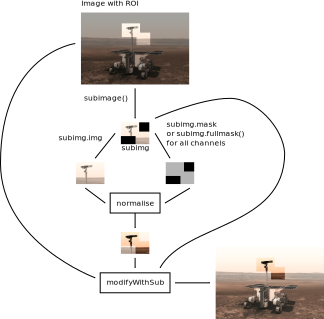
\includegraphics[width=5in]{norm.pdf}
\caption{The image processing in the norm node}
\label{norm.pdf}
\end{figure}
\clearpage
Finally, if the node was not enabled we set \texttt{node.img} (our output)
to be the input image:
\begin{lstlisting}
            else:
                node.img = img
\end{lstlisting}
and output the image to the node's zeroth (and only) output:
\begin{lstlisting}
        node.setOutput(0, node.img)
\end{lstlisting}




%\bibliographystyle{plain}
%\bibliographystyle{alpha}
%\bibliography{bib}
%\printbibliography

\end{document}
